\documentclass[11pt]{article}
\usepackage[margin=1in]{geometry}
\usepackage{amsmath,amssymb,booktabs,graphicx,float,caption,subcaption}
\usepackage[hidelinks]{hyperref}
\hypersetup{pdftitle={Fault-versus-Event Anomaly Discrimination in Correlated Sensor Streams},
            pdfauthor={Team Signal or Noise}}
\setlength{\parskip}{4pt}
\captionsetup{font=small}
\graphicspath{{figures/}}

\title{\textbf{Fault-versus-Event Anomaly Discrimination in Correlated Sensor Streams\\using Unsupervised Detectors and Spatial Correlation Features}\\[4pt]
\large CSE 575 Statistical Machine Learning, Fall 2026 \;|\; Topic P12: Anomaly Detection \;|\; Team \emph{Signal or Noise}}
\author{Manav \and Rashi Sharma \and Karthik Ponugoti \and Harsh Tita \and Tejas Rajaram Uttare \and Ziyad Jafarulla Parkar}
\date{December 2026}

\begin{document}
\maketitle

\begin{abstract}
An unusual reading from a sensor network can be a real environmental \emph{event} or an instrument \emph{failure}. Standard anomaly detectors flag both and cannot tell them apart. On the Intel Berkeley Lab deployment (54 nodes, 2.3 million readings) we implement five detectors from scratch (KNN distance, K-means, a Gaussian mixture fitted by EM, PCA/SVD reconstruction error and a Gaussian HMM), compare them with a $k$-standard-deviation baseline on synthetic anomalies with known labels, and then classify every detected anomaly as event or failure with our own Naive Bayes and logistic regression, using spatial agreement with neighbouring nodes, battery telemetry and cross-channel consistency. Models that use cross-node structure or time order do best: PCA reaches AUC $0.859$ and the HMM $0.843$ against $0.746$ for the baseline (5/5 folds better). With first-difference features GMM and KNN reach $0.946$ and $0.921$. On PCA-flagged anomalies, logistic regression keeps $97.7\%$ of event alerts while removing $95.0\%$ of failure alerts; replacing spatial neighbours with random ones lowers failure recall to $88.3\%$. We also report negative results: stuck-at failures are invisible to every detector, EM imputation does not improve detection, and battery voltage alone predicts imminent failure as well as our multi-feature model.
\end{abstract}

\section{Problem}
Topic P12 asks how to find rare or unusual instances in data, as studied for auction fraud~\cite{netprobe}, categorical data~\cite{akoglu} and rare categories~\cite{he}. In a wireless sensor network an unusual reading has two very different causes. A \textbf{genuine event} (a door opening, HVAC cycling, sunlight reaching a window) is what the network was deployed to observe. An \textbf{instrument failure} (a degrading node emitting unreliable values) is a maintenance task. Distance-, density- and reconstruction-based detectors cannot separate them, because both are rare and far from the bulk of the data.

Our hypothesis is that the two can be separated with information the detectors ignore: a real event also appears at nearby nodes, while a failing sensor's anomaly is confined to one node and often coincides with low battery. The project therefore has two stages: \emph{detect} anomalies, then \emph{classify} each one as event or failure.

\section{Data}
We use the Intel Berkeley Research Lab dataset~\cite{intel}, provided with the course materials under topic P4 and permitted for P12: 54 nodes recording temperature, humidity, light and battery voltage every 31 seconds from 28 February to 5 April 2004, about 2.3 million readings, with node coordinates in metres. The same deployment was used for distributed regression~\cite{guestrin} and model-driven acquisition~\cite{deshpande}.

\textbf{Preparation.} We average 10 epochs into one step ($\approx$5 minutes), giving a tensor of 9{,}940 steps $\times$ 54 nodes $\times$ 4 channels. Three properties of the raw data shaped the pipeline:
\begin{itemize}\itemsep1pt
\item \textbf{The epoch counter is 16-bit and resets} around 21 March, so the time grid is built from timestamps, not epochs.
\item \textbf{27.3\% of (step, node) cells are missing}; 16.6\% before 20 March.
\item \textbf{Most nodes fail late in the deployment.} 51 of 54 nodes eventually drop below 2.3~V, and 21.7\% of observed temperature and 16.7\% of humidity readings are physically impossible (e.g.\ 120\,$^\circ$C). After 20 March, 80\% of observed cells are already failing (Fig.~\ref{fig:profile}).
\end{itemize}
Out-of-range readings are kept on load, since they are the failure class we study. Injected-anomaly experiments use the period before 2004-03-20 (5{,}842 steps); the late period is used for the real-failure (weak-label) evaluation.

\begin{figure}[H]
\centering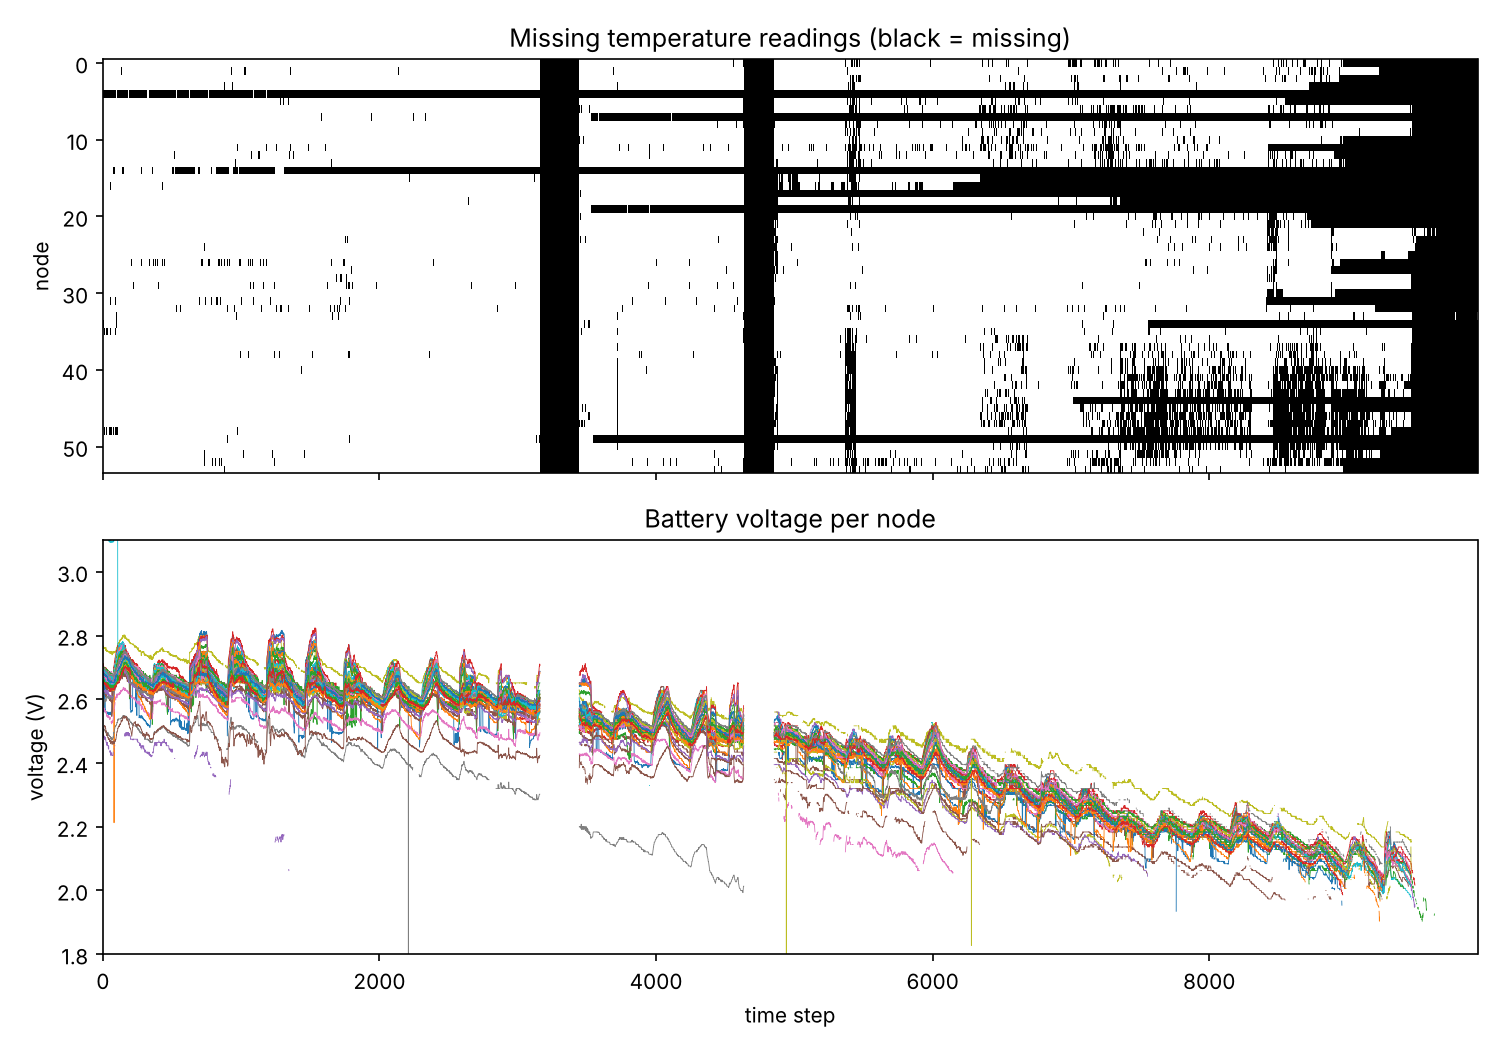
\includegraphics[width=0.85\linewidth]{missing_and_voltage.png}
\caption{Missing temperature readings per node (top) and battery voltage per node (bottom) over the deployment.}
\label{fig:profile}
\end{figure}

\section{Method}
All detectors, the imputer, both classifiers and all metrics are our own NumPy/SciPy implementations of the course methods~\cite{bishop} (no scikit-learn or HMM libraries).

\subsection{Preprocessing}
Each fold is imputed and standardised separately using only its training window: robust z-scores per node and channel (median and $1.4826\times$MAD, so failing sensors in the training window do not inflate the scale). Detectors see temperature, humidity and light; voltage drifts steadily as batteries drain and would dominate any z-score, so it is used only in Stage C.

\subsection{Stage A: detectors}
Every detector implements \texttt{fit(X)} and \texttt{score(X)} on a $(T, N, C)$ tensor and returns a $(T, N)$ anomaly score.
\begin{itemize}\itemsep1pt
\item \textbf{$k$-sigma baseline}: largest absolute z-score across channels.
\item \textbf{KNN distance}: Euclidean distance to the $k$-th nearest training point (subsampled reference set, chunked computation).
\item \textbf{K-means}: Lloyd's algorithm with k-means++ initialisation and restarts; score = distance to the nearest centroid.
\item \textbf{GMM / EM}: full-covariance Gaussian mixture fitted by EM with log-sum-exp responsibilities and a ridge; score = negative log-likelihood; $K$ chosen by BIC.
\item \textbf{PCA / SVD}: each time step is a vector over all nodes and channels; SVD of the centred training matrix; score = per-node squared reconstruction error from the top-$k$ components. A building-wide change is explained by the top components, while one node disagreeing with its correlated neighbours is not.
\item \textbf{HMM}: Gaussian-emission HMM (diagonal covariances) trained per node by Baum--Welch with scaled forward--backward; score = $-\log p(x_t \mid x_{1:t-1})$.
\end{itemize}

\subsection{Stage B: missing data}
EM for a multivariate Gaussian over the nodes of each channel, exploiting the correlation between co-evolving series~\cite{cai}: the E-step fills each missing entry with $\mathbb{E}[x_m\mid x_o]=\mu_m+\Sigma_{mo}\Sigma_{oo}^{-1}(x_o-\mu_o)$ and adds the conditional covariance; the M-step re-estimates $\mu,\Sigma$. Physically impossible values and $|z|>4$ outliers are hidden from the model. Quality is measured by hiding 10\% of observed values in runs of 1, 6 or 24 steps and scoring recovery.

\subsection{Stage C: event vs failure}
For each flagged cell $(t,n)$ we compute five features: \textbf{neighbour agreement} (fraction of the 4 spatially nearest nodes whose detector score also exceeds the threshold within $t\pm2$ steps); \textbf{battery level} and \textbf{battery slope} over the previous 12 steps; \textbf{temperature-residualised voltage} (voltage minus a per-node linear fit on temperature, since voltage varies with temperature); and \textbf{cross-channel consistency} (correlation of temperature and humidity changes over the last 6 steps). We train Gaussian Naive Bayes and L2-regularised logistic regression (gradient descent) on these features.

\subsection{Stage D: failure prediction}
For each node, at every healthy observed step we use voltage level, voltage slope over 12 steps, temperature-residualised voltage and temperature to predict whether the node's first real failure occurs within the next $H$ steps ($\approx$1\,h, 6\,h, 1 day), with leave-nodes-out cross-validation.

\section{Evaluation protocol}
\textbf{Labels.} The data are unlabelled, so we inject synthetic anomalies into the standardised test window. \emph{Events} raise temperature and light and lower humidity, with a smooth ramp, at a node and its 4 neighbours (neighbours at 0.7 of the amplitude). \emph{Failures} add independent noise to one node's temperature and humidity and drop its voltage. Harder variants: lagged events, stuck-at sensors and slow drift. Separately, cells with collapsed voltage or impossible values serve as weak labels for real failures.

\textbf{Protocol.} Five contiguous temporal folds with a 12-step gap on each side of the test block, so adjacent readings do not leak. Only observed cells that are not already real anomalies are scored. Default injection: 10 events and 10 failures per fold at 4 training standard deviations, repeated over 10 seeds.

\textbf{Metrics.} ROC AUC (overall, events vs normal, failures vs normal) and precision@$k$ with $k$ the number of anomalous cells for detection; accuracy, balanced accuracy and confusion matrices for event vs failure. Runs within a fold share data, so confidence intervals and paired $t$-tests against the baseline use the 5 fold means.

\section{Results}

\subsection{Detection}
Table~\ref{tab:det} and Fig.~\ref{fig:cv} summarise 50 runs per detector. PCA (+0.113 AUC, 95\% CI [+0.031, +0.196], $p=0.019$) and the HMM (+0.097, [+0.046, +0.147], $p=0.006$) beat the baseline on all 5 folds. Their gain comes almost entirely from \emph{events} (+0.130 and +0.106), which is where a per-node threshold struggles. KNN and GMM on raw channels are statistically indistinguishable from the baseline, and K-means is worse ($-0.044$, $p=0.043$). Failures are easy for every method (AUC $\ge 0.885$).

\begin{table}[H]
\centering\small
\begin{tabular}{lccccc}
\toprule
Detector & AUC & 95\% CI & AUC events & AUC failures & precision@$k$\\
\midrule
$k$-sigma (baseline) & 0.746 $\pm$ 0.095 & [0.635, 0.857] & 0.716 & 0.919 & 0.274\\
KNN distance & 0.763 $\pm$ 0.070 & [0.679, 0.847] & 0.736 & 0.917 & 0.084\\
K-means & 0.702 $\pm$ 0.098 & [0.582, 0.822] & 0.670 & 0.885 & 0.063\\
GMM / EM & 0.750 $\pm$ 0.099 & [0.627, 0.873] & 0.719 & 0.924 & 0.083\\
PCA / SVD & \textbf{0.859} $\pm$ 0.042 & [0.823, 0.896] & \textbf{0.846} & 0.936 & \textbf{0.385}\\
HMM & 0.843 $\pm$ 0.058 & [0.771, 0.914] & 0.822 & \textbf{0.960} & 0.262\\
\bottomrule
\end{tabular}
\caption{Detection on injected anomalies (magnitude 4, 10 seeds $\times$ 5 folds). Mean $\pm$ std over runs; CI over fold means.}
\label{tab:det}
\end{table}

\begin{figure}[H]
\centering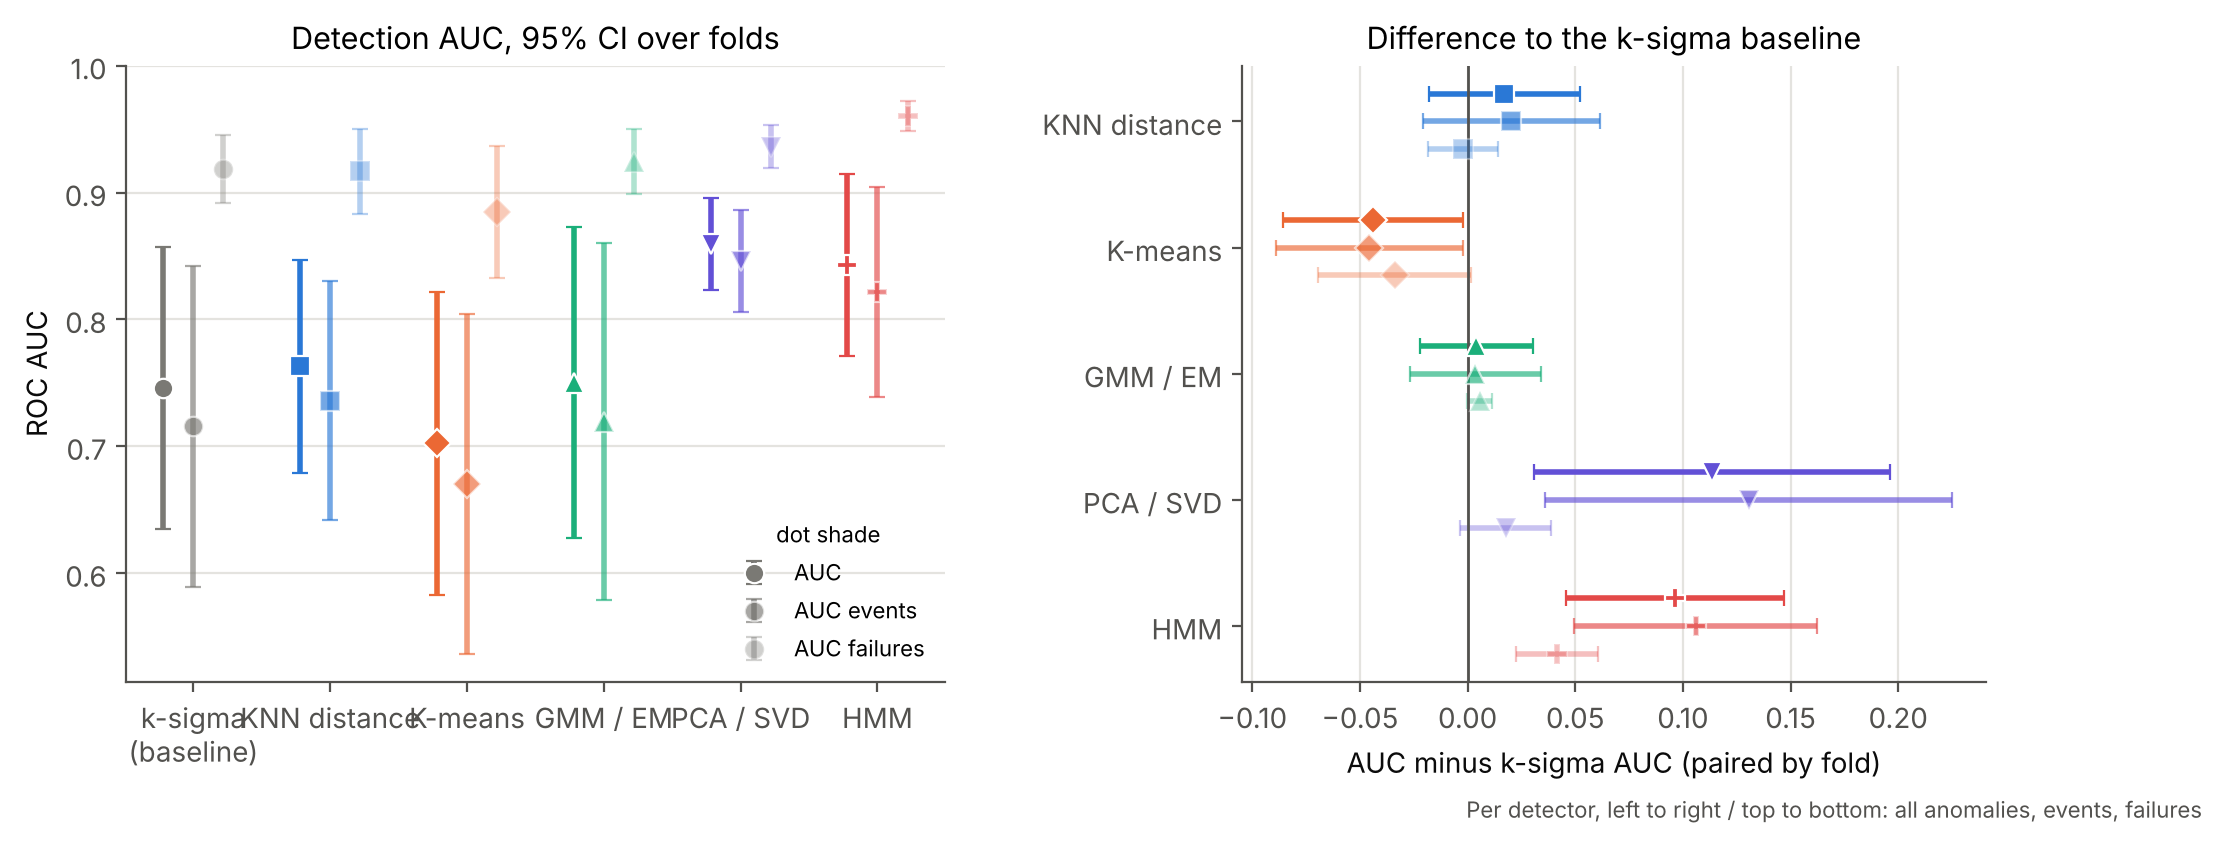
\includegraphics[width=\linewidth]{repeated_cv.png}
\caption{Left: AUC with 95\% CI over folds (dark: all anomalies, mid: events, light: failures). Right: paired difference to the $k$-sigma baseline.}
\label{fig:cv}
\end{figure}

\textbf{Hyper-parameters.} PCA works best with $k=5$ components (AUC 0.862 vs 0.756 for $k=1$ and 0.780 for $k=50$); the first two components already explain $\approx$97\% of the variance, so too few components miss local structure and too many reconstruct the anomaly itself. Per-node HMMs beat a single shared HMM at every state count (e.g.\ 0.858 vs 0.801 at $S=4$), and AUC rises slowly with $S$ (0.822 at $S=2$ to 0.872 at $S=6$).

\textbf{Feature engineering.} Adding first differences in time (\texttt{channels+diff}) changes the picture for the point-wise detectors (Fig.~\ref{fig:feat}): KNN rises from 0.781 to 0.896 (0.921 with features clipped at 6), and GMM from 0.767 to 0.933 (0.946 clipped, 5/5 folds better than the baseline, $p=0.003$). K-means gains less (0.729 to 0.787). These settings were selected on the same folds they are reported on, so they are optimistic; we report them separately from Table~\ref{tab:det}.

\begin{figure}[H]
\centering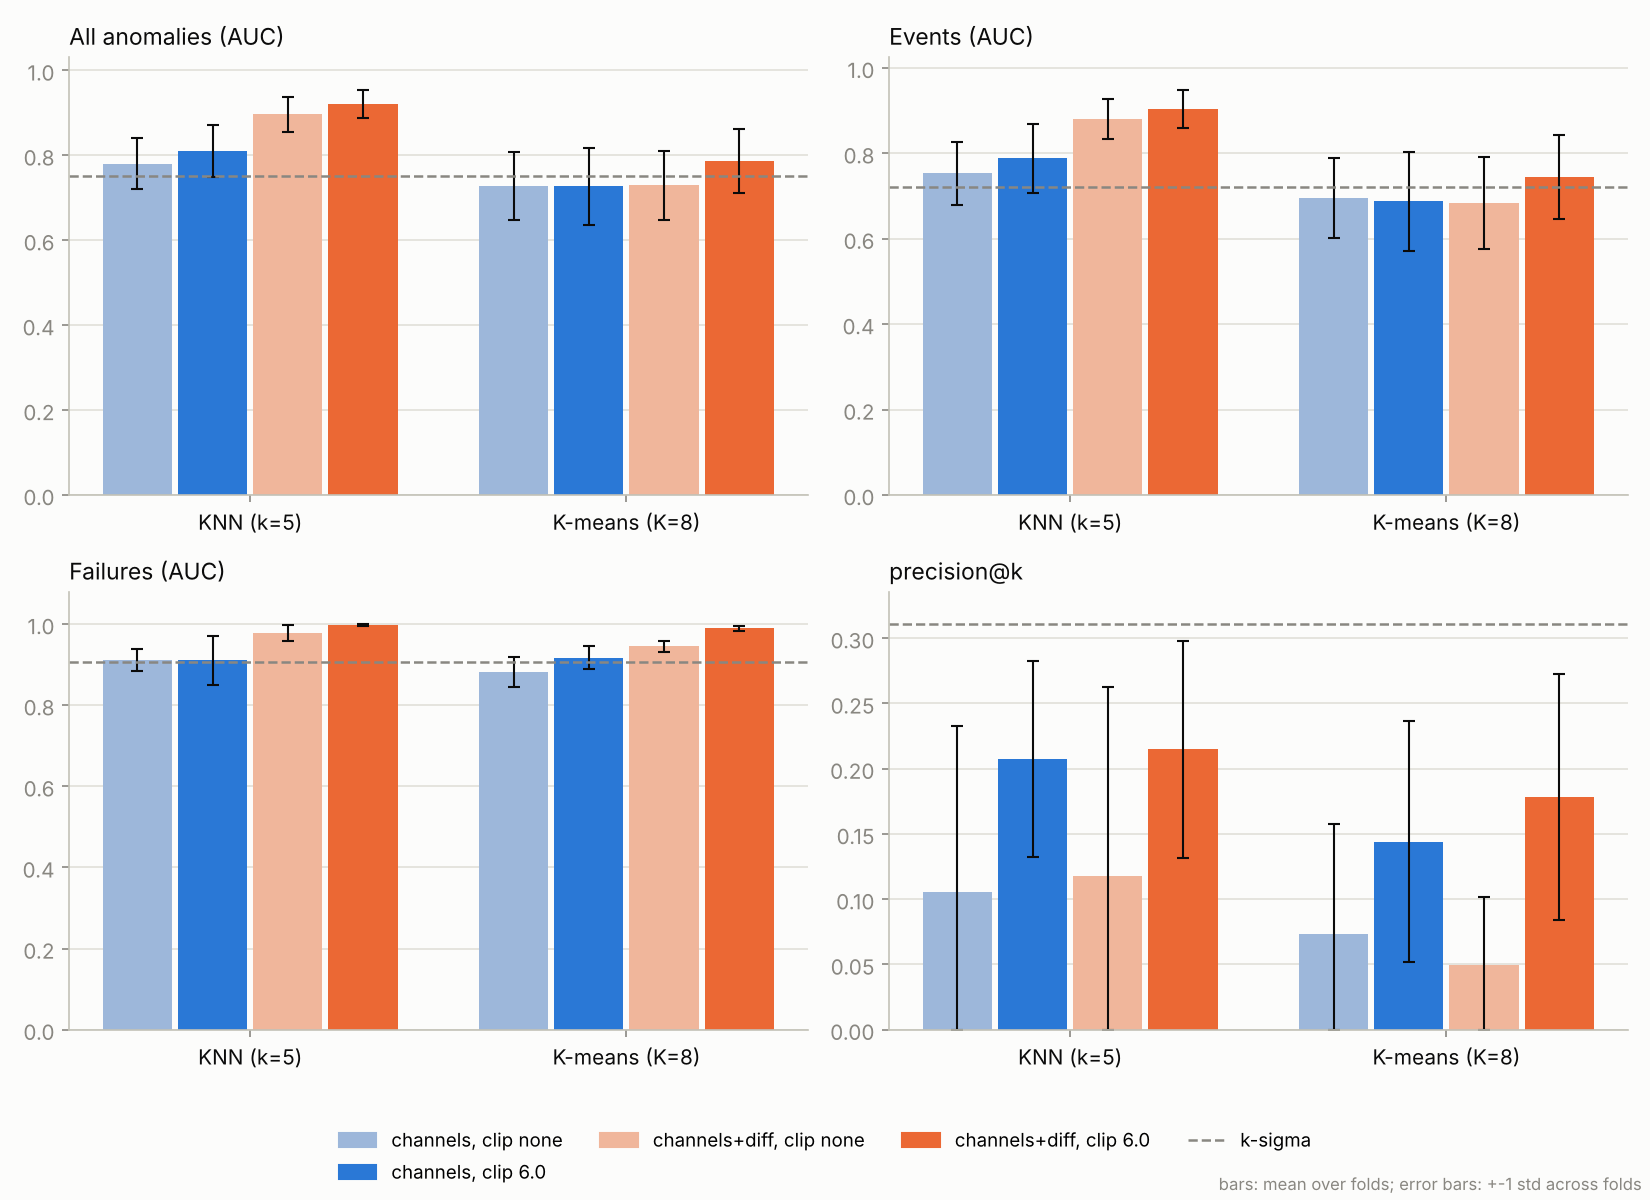
\includegraphics[width=0.78\linewidth]{features.png}
\caption{KNN and K-means with raw channels vs channels plus first differences, with and without clipping at 6. Dashed line: $k$-sigma.}
\label{fig:feat}
\end{figure}

\subsection{Difficulty and anomaly kinds}
AUC grows with magnitude for every detector (Fig.~\ref{fig:mag}); at 1 SD only the HMM (0.629) and PCA (0.596) are clearly above chance. Table~\ref{tab:kinds} breaks results down by anomaly kind. Lagged events are as easy as synchronous ones. \textbf{Stuck-at failures are not detected by any method} (AUC $\approx$0.50, and below 0.5 in quiet periods), because a constant value is not unusual to a detector that looks at levels; slow drift is detected only moderately. Placing events in quiet periods hurts the threshold and point-wise detectors but not PCA (0.861), which models cross-node structure.

\begin{figure}[H]
\centering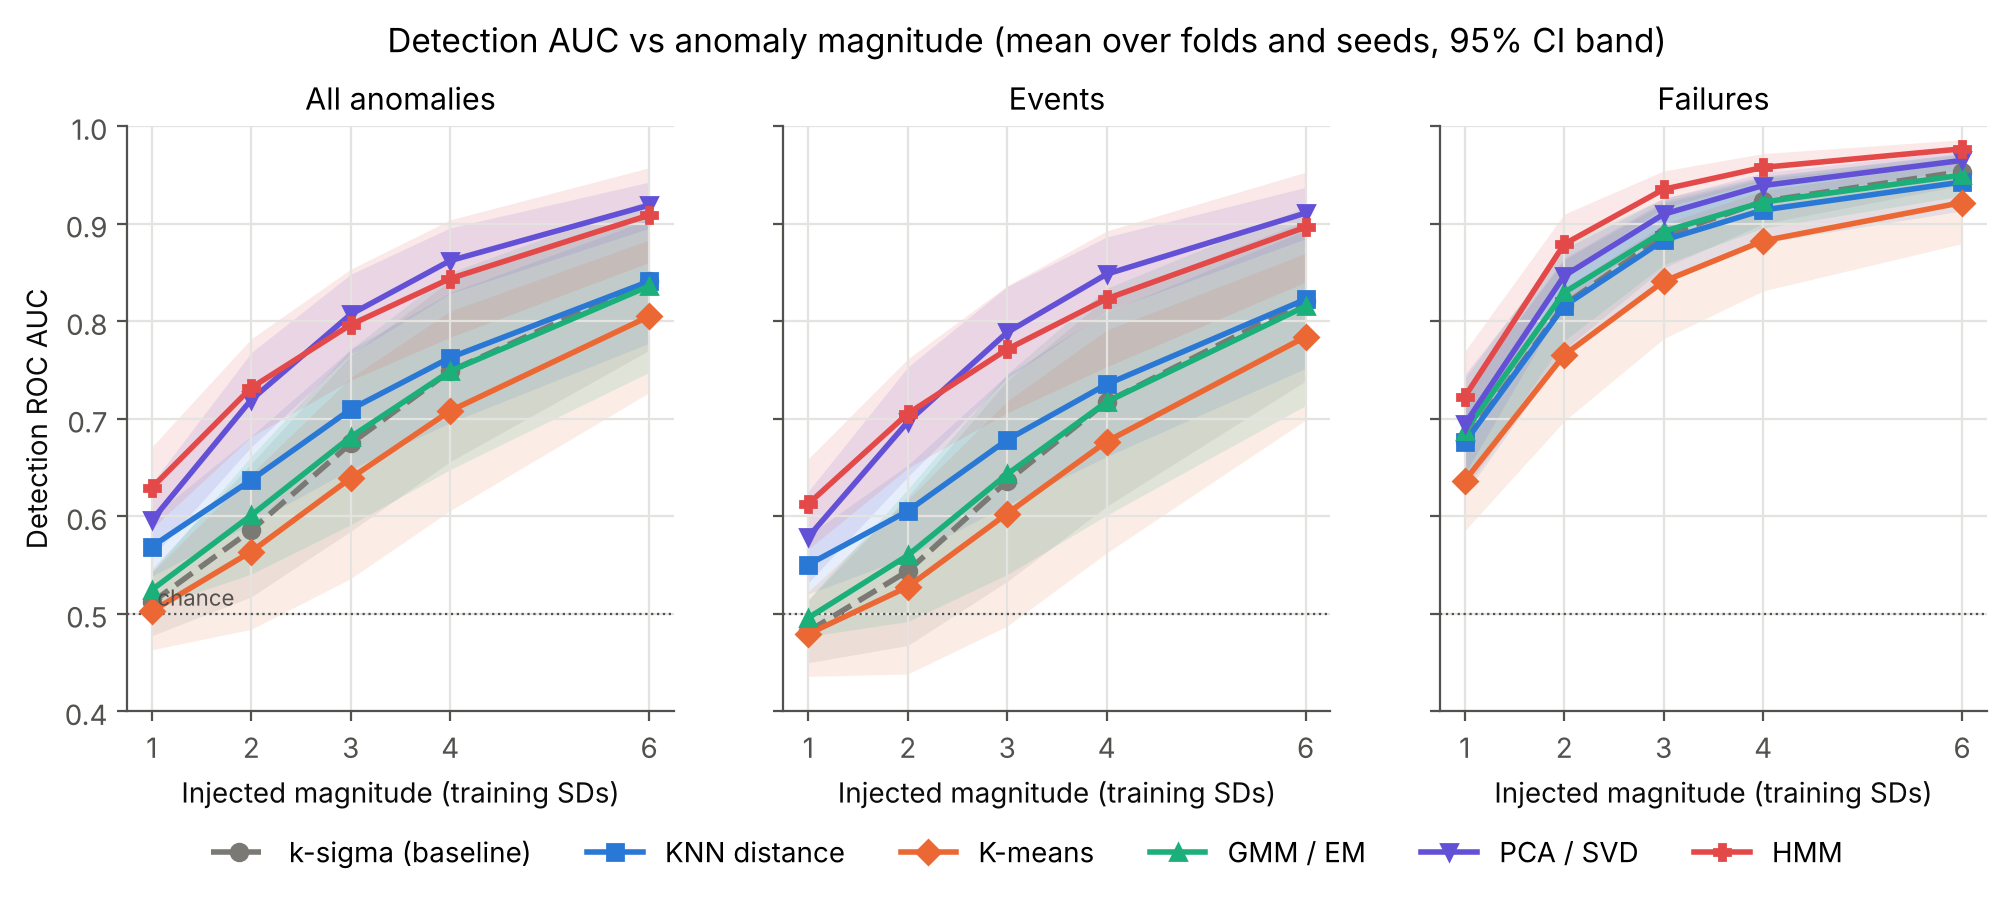
\includegraphics[width=\linewidth]{magnitude_sweep.png}
\caption{Detection AUC vs injected magnitude (5 seeds per point, 95\% CI band).}
\label{fig:mag}
\end{figure}

\begin{table}[H]
\centering\small
\begin{tabular}{llcccccc}
\toprule
Placement & Kind & $k$-sigma & KNN & K-means & GMM & PCA & HMM\\
\midrule
anywhere & event & 0.714 & 0.734 & 0.661 & 0.711 & \textbf{0.844} & 0.823\\
 & lagged event & 0.715 & 0.732 & 0.661 & 0.709 & \textbf{0.848} & 0.820\\
 & noise failure & 0.909 & 0.918 & 0.885 & 0.926 & 0.926 & \textbf{0.962}\\
 & stuck-at & 0.527 & 0.500 & 0.508 & 0.512 & 0.527 & 0.499\\
 & slow drift & 0.731 & 0.764 & 0.718 & \textbf{0.777} & 0.746 & 0.771\\
\midrule
quiet & event & 0.635 & 0.665 & 0.602 & 0.648 & \textbf{0.861} & 0.787\\
 & stuck-at & 0.393 & 0.330 & 0.380 & 0.338 & 0.419 & 0.343\\
 & slow drift & 0.664 & 0.700 & 0.661 & 0.718 & 0.722 & \textbf{0.724}\\
\bottomrule
\end{tabular}
\caption{AUC per anomaly kind (each kind injected alone, magnitude 4, 3 seeds).}
\label{tab:kinds}
\end{table}

\subsection{Missing data}
On clean readings, EM imputation recovers long gaps much better than forward fill (24-step outages: temperature RMSE 0.62 vs 1.58\,$^\circ$C, humidity 1.06 vs 2.42\%), while forward fill wins on isolated single-step holes (0.28 vs 0.65\,$^\circ$C) because adjacent readings are nearly identical (Fig.~\ref{fig:mask}). On raw data with failing sensors, forward fill wins almost everywhere, since failing sensors repeat absurd values that a model of the neighbours cannot predict. Using EM instead of forward fill inside the detection bench did \emph{not} help: PCA fell from 0.862 to 0.813 and the other detectors changed by at most 0.02. Smooth conditional means likely blur the sharp local deviations the detectors look for. Forward fill remains our default.

\begin{figure}[H]
\centering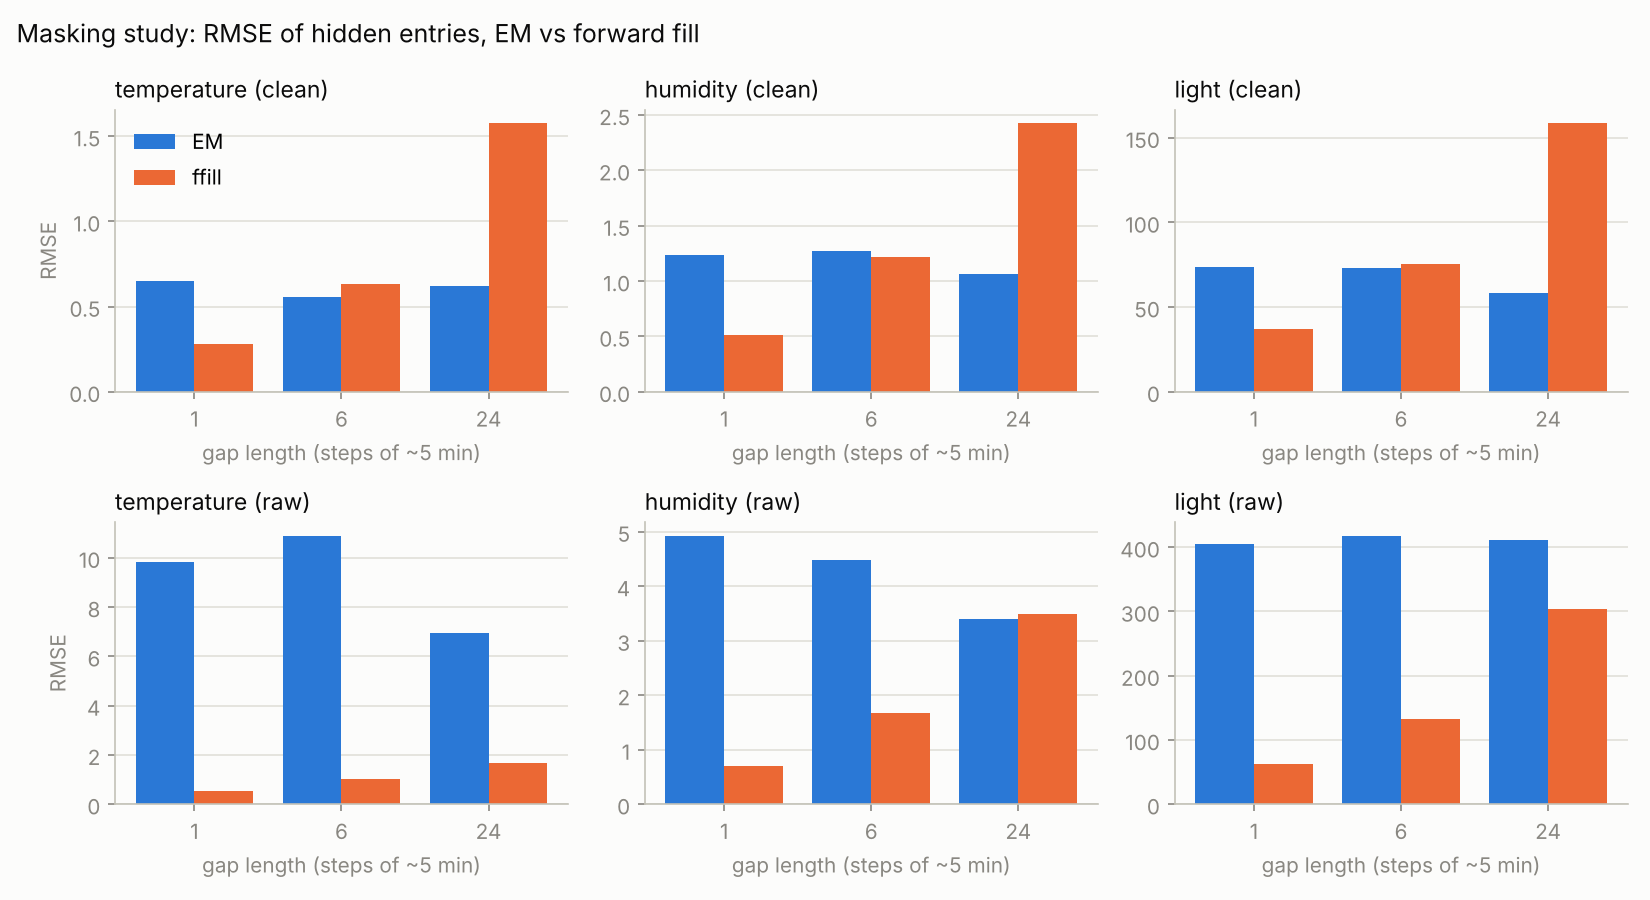
\includegraphics[width=0.8\linewidth]{masking_rmse.png}
\caption{Imputation RMSE per channel, EM vs forward fill, for outages of 1, 6 and 24 steps.}
\label{fig:mask}
\end{figure}

\subsection{Event vs failure}
Classifiers are trained on anomalies injected into the training window and tested on those flagged in the test window (top-$k$ cells of the detector), 5 seeds $\times$ 5 folds. Table~\ref{tab:abl} shows the PCA-flagged results; Fig.~\ref{fig:conf} the confusion matrices.

\begin{table}[H]
\centering\small
\begin{tabular}{lcccc}
\toprule
 & \multicolumn{2}{c}{Naive Bayes} & \multicolumn{2}{c}{Logistic regression}\\
Condition & bal.\ acc. & $\Delta$ & bal.\ acc. & $\Delta$\\
\midrule
all features & 0.914 & --- & \textbf{0.957} & ---\\
drop neighbour agreement & 0.940 & +0.026 & 0.928 & $-0.029$ ($p$ 0.027)\\
drop battery level & 0.895 & $-0.019$ & 0.961 & +0.005\\
drop battery slope & 0.911 & $-0.003$ & 0.952 & $-0.005$\\
drop residual voltage & 0.914 & 0.000 & 0.957 & +0.001\\
drop cross-channel consistency & 0.898 & $-0.016$ & 0.918 & $-0.039$ ($p$ 0.025)\\
only neighbour agreement & 0.885 & $-0.029$ & 0.885 & $-0.071$ ($p$ 0.019)\\
random neighbours (control) & 0.861 & $-0.053$ & 0.926 & $-0.031$ ($p$ 0.065)\\
\bottomrule
\end{tabular}
\caption{Event-vs-failure balanced accuracy on PCA-flagged anomalies, standard injection. $\Delta$: paired by fold against all features.}
\label{tab:abl}
\end{table}

\begin{figure}[H]
\centering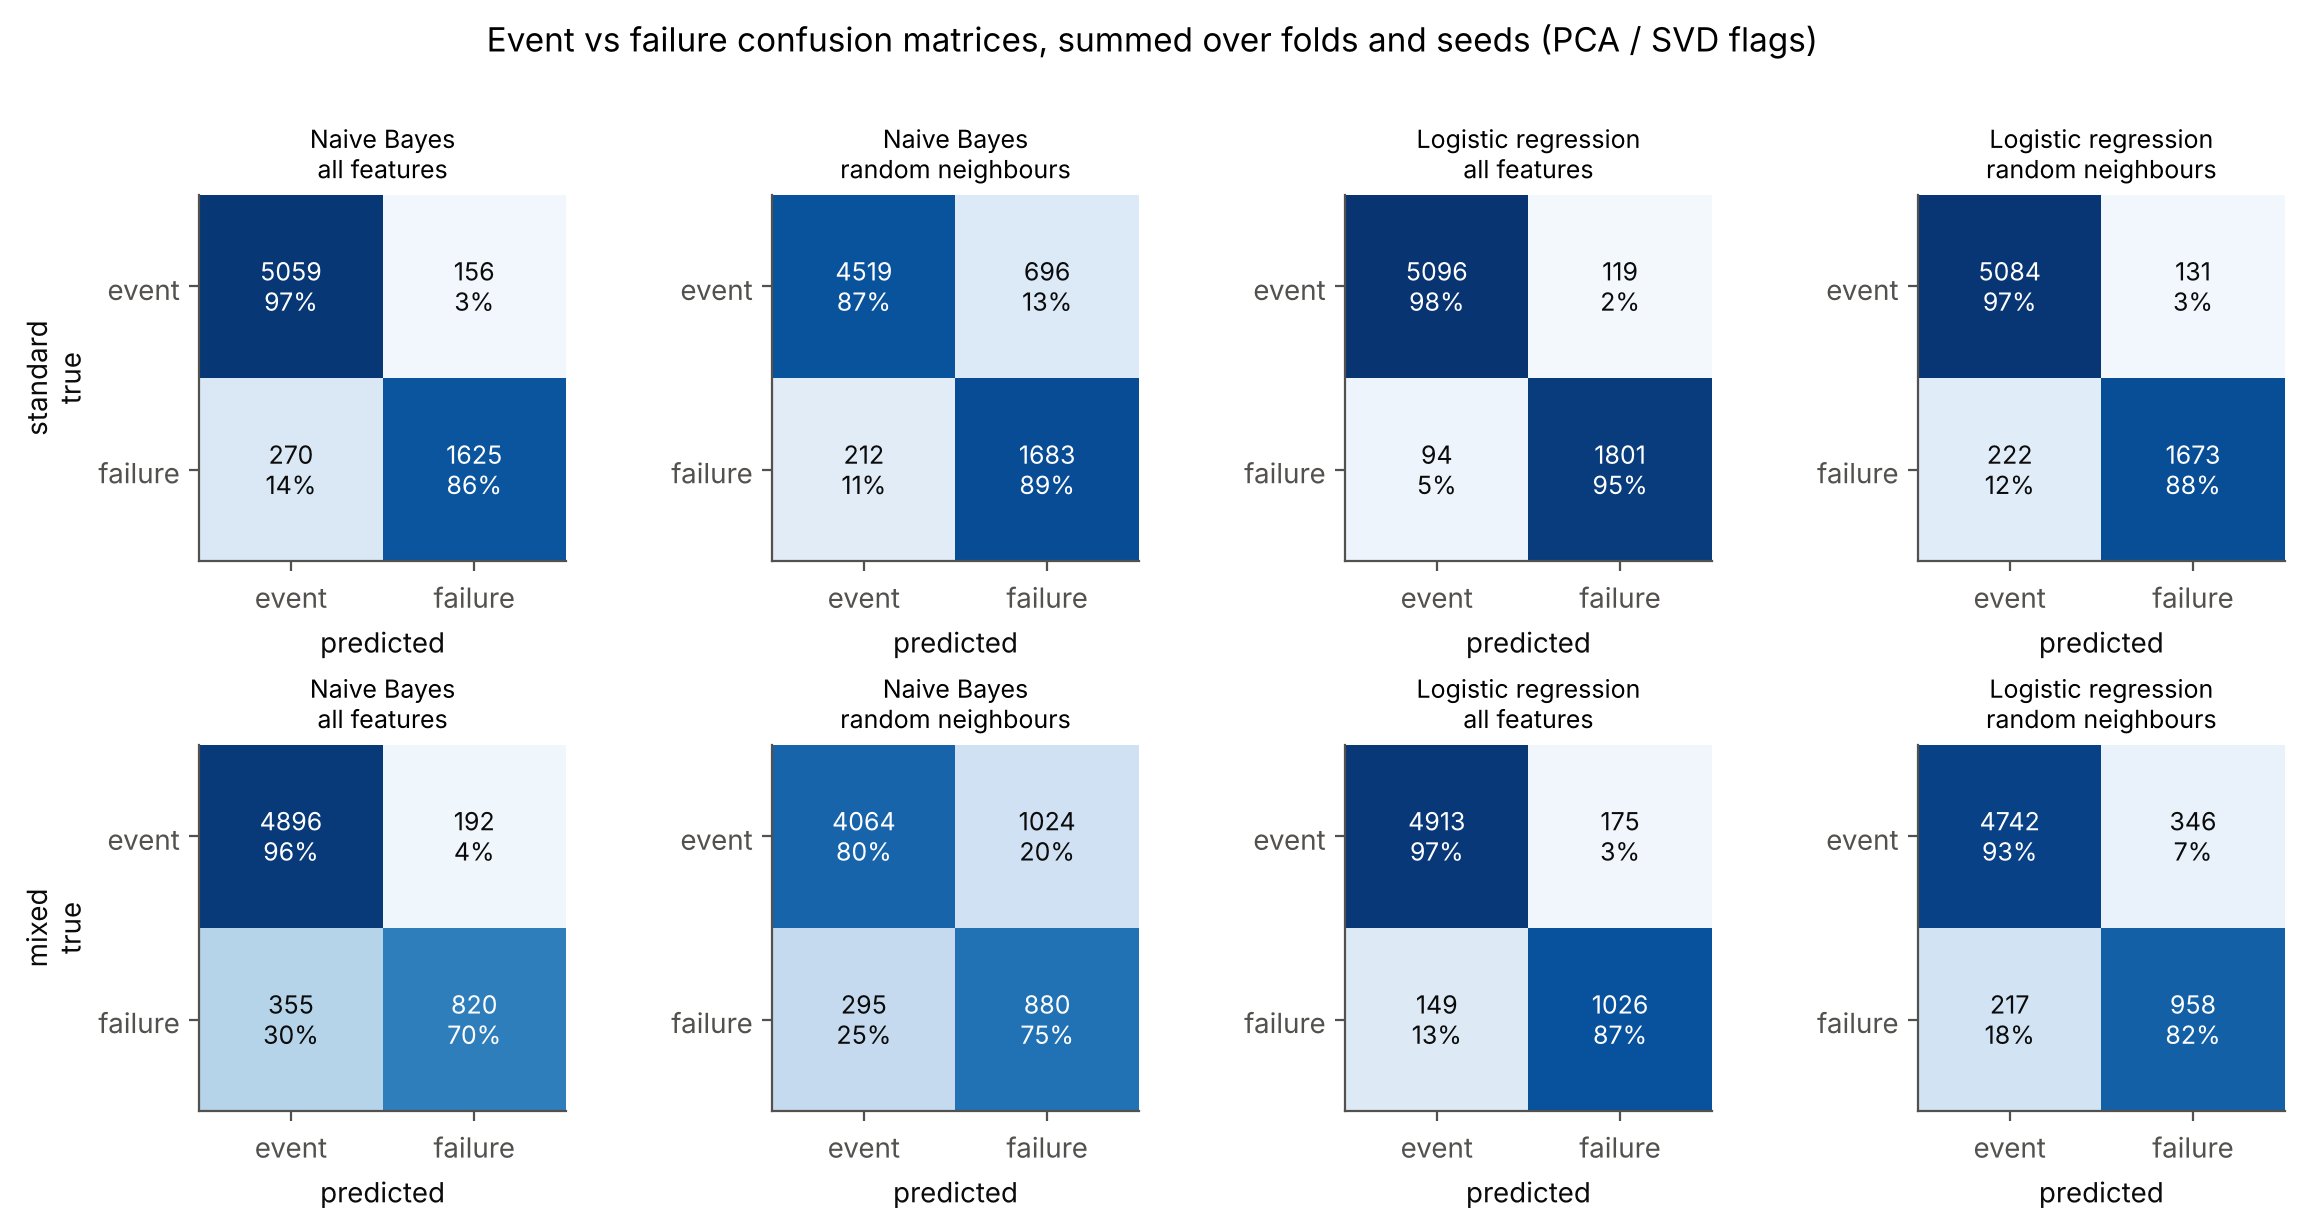
\includegraphics[width=\linewidth]{confusion_pca.png}
\caption{Confusion matrices summed over folds and seeds (PCA flags). Top: standard injection; bottom: mixed injection with lagged events, stuck-at and drift.}
\label{fig:conf}
\end{figure}

\textbf{False-alarm reduction.} With PCA flags and logistic regression, filtering out alerts classified as failures removes 95.0\% of failure alerts (1{,}801 of 1{,}895) while keeping 97.7\% of event alerts (5{,}096 of 5{,}215), i.e.\ 27\% fewer alerts with almost no loss of real events. With random neighbours instead of spatial ones, failure removal drops to 88.3\% (logistic regression) and event retention to 86.7\% (Naive Bayes), so the spatial structure itself carries information, not just the extra feature. On the harder mixed injection the full model still keeps 96.6\% of events and removes 87.3\% of failures.

\textbf{Which features matter.} For logistic regression, neighbour agreement and cross-channel consistency are the features whose removal significantly hurts. The battery features add almost nothing on top of them, partly because the synthetic failures are already separable by their single-node, incoherent pattern. Naive Bayes does slightly \emph{better} without neighbour agreement, which we attribute to its independence assumption double-counting information shared by neighbour agreement and cross-channel consistency.

\subsection{Real failures (weak labels)}
Detectors fitted on the healthy period and scored on the late period separate weakly labelled failing cells from the rest with AUC 0.944--0.977 (GMM 0.977, HMM 0.976, KNN 0.975, baseline 0.973, PCA 0.944). This task is easy because 71\% of the observed late-period cells hold physically impossible values; it confirms the detectors respond to real failures but does not discriminate between them.

\subsection{Predicting failure (Stage D)}
Voltage history predicts a node's first failure well ahead of time: leave-nodes-out AUC is 0.941 one hour ahead, 0.948 six hours ahead and 0.969 one day ahead (Fig.~\ref{fig:staged}). However, voltage level alone is equally good (0.952, 0.948, 0.961): in this deployment the battery level, not its trajectory, is the leading indicator.

\begin{figure}[H]
\centering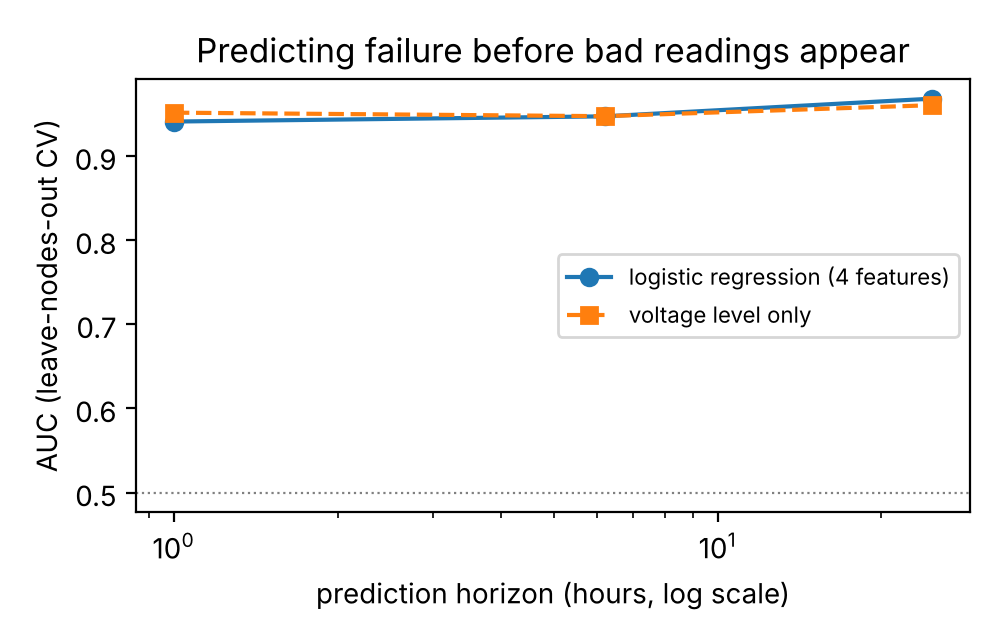
\includegraphics[width=0.55\linewidth]{stage_d_auc.png}
\caption{Failure prediction AUC vs horizon, logistic regression vs voltage level alone.}
\label{fig:staged}
\end{figure}

\section{Discussion and limitations}
\begin{itemize}\itemsep1pt
\item \textbf{Structure beats distance.} The detectors that model cross-node correlation (PCA) or time order (HMM, or first-difference features) are the ones that find events; point-wise models of raw levels are no better than a threshold.
\item \textbf{Synthetic labels.} Event-vs-failure accuracy is measured on our own injected anomalies, whose failure model (single node, incoherent, voltage drop) matches our features. Real failures in this dataset are dominated by impossible values, which are easier still. A labelled set of real events would be the main next step.
\item \textbf{Stuck-at sensors} need a different detector (e.g.\ variance or rate-of-change over a window); none of ours sees them.
\item \textbf{Tuning on reported folds.} Feature clipping and \texttt{channels+diff} were chosen on the same folds; a nested split would give unbiased estimates.
\item \textbf{Small number of folds.} With 5 folds the exact sign-flip test cannot go below $p=0.0625$; we therefore also report $t$-tests and fold win counts.
\end{itemize}

\section{Conclusion}
Spatial and temporal structure are what separate genuine events from sensor failures. PCA and the HMM detect injected events significantly better than a $k$-sigma threshold, and a simple logistic regression on neighbour agreement and cross-channel consistency filters out 95\% of failure alerts while keeping 98\% of events. Replacing real neighbours with random ones degrades this, supporting our hypothesis. The negative results (stuck-at sensors, EM imputation, battery trajectory) are equally informative about where the approach stops working.

\section*{Team contributions}
\begin{tabular}{ll}
\toprule
Member & Contribution\\
\midrule
Manav & Data pipeline, harness, integration, weak-label and Stage D evaluation\\
Rashi Sharma & KNN and K-means detectors, feature and clipping study\\
Karthik Ponugoti & PCA/SVD and HMM detectors, component and state sweeps\\
Harsh Tita & GMM/EM detector, EM imputation, masking study\\
Tejas Rajaram Uttare & Stage C features, Naive Bayes and logistic regression\\
Ziyad Jafarulla Parkar & Injection variants, repeated CV, statistics, ablation, figures\\
\bottomrule
\end{tabular}

Slides and this report are shared work. All code was cross-reviewed in pull requests.

\section*{Code declaration}
\textbf{Our code}: everything in \texttt{src/signoise/} and \texttt{scripts/} of our repository: data loading and preprocessing, all six detectors, EM imputation, both classifiers, all metrics (ROC AUC via the Mann--Whitney statistic, precision/recall, confusion matrices), anomaly injection, cross-validation and statistics. \textbf{Third-party} (used under their open-source licences, not submitted): NumPy and SciPy for array operations and linear algebra, pandas for loading and tables, matplotlib for figures, pytest for tests. No machine learning library was used for any method.

\textbf{Use of AI tools.} [Team to confirm before submission: describe here whether and how AI coding assistants were used, per the course policy.]

\begin{thebibliography}{9}\small
\bibitem{netprobe} S.~Pandit, D.~H.~Chau, S.~Wang and C.~Faloutsos. NetProbe: A fast and scalable system for fraud detection in online auction networks. WWW, 2007, pp.~201--210.
\bibitem{akoglu} L.~Akoglu, H.~Tong, J.~Vreeken and C.~Faloutsos. Fast and reliable anomaly detection in categorical data. CIKM, 2012, pp.~415--424.
\bibitem{he} J.~He, H.~Tong and J.~G.~Carbonell. Rare category characterization. ICDM, 2010, pp.~226--235.
\bibitem{intel} P.~Bodik, W.~Hong, C.~Guestrin, S.~Madden, M.~Paskin and R.~Thibaux. Intel Lab Data, 2004. \url{http://db.csail.mit.edu/labdata/labdata.html}
\bibitem{guestrin} C.~Guestrin, P.~Bod\'ik, R.~Thibaux, M.~Paskin and S.~Madden. Distributed regression: an efficient framework for modeling sensor network data. IPSN, 2004, pp.~1--10.
\bibitem{deshpande} A.~Deshpande, C.~Guestrin, S.~Madden, J.~M.~Hellerstein and W.~Hong. Model-driven data acquisition in sensor networks. VLDB, 2004, pp.~588--599.
\bibitem{cai} Y.~Cai, H.~Tong, W.~Fan and P.~Ji. Fast mining of a network of coevolving time series. SDM, 2015.
\bibitem{bishop} C.~M.~Bishop. \emph{Pattern Recognition and Machine Learning}. Springer, 2006.
\end{thebibliography}
\end{document}
